% =====================================================================
%  Machine verification and certification of research mathematics
%  Jeppe Rich, DTU Management
%  Compile:  latexmk -pdf verification_talk.tex
% =====================================================================
\documentclass[aspectratio=169,11pt]{beamer}

\usetheme{default}
\usecolortheme{default}
\setbeamertemplate{navigation symbols}{}
\setbeamertemplate{itemize items}[circle]

\usepackage[T1]{fontenc}
\usepackage[utf8]{inputenc}
\usepackage{lmodern}
\usepackage{amsmath,amssymb}
\usepackage{booktabs}
\usepackage{graphicx}
\usepackage{xcolor}
\usepackage{array}

% ---- palette --------------------------------------------------------
\definecolor{ink}{HTML}{12202C}
\definecolor{dtured}{HTML}{990000}
\definecolor{okgreen}{HTML}{2E7D32}
\definecolor{badred}{HTML}{B23A2E}
\definecolor{flagamber}{HTML}{9A7413}
\definecolor{slate}{HTML}{5A6B7A}
\definecolor{panel}{HTML}{F2F4F6}

\setbeamercolor{structure}{fg=dtured}
\setbeamercolor{normal text}{fg=ink}
\setbeamercolor{frametitle}{fg=ink}
\setbeamerfont{frametitle}{size=\large,series=\bfseries}
\setbeamercolor{block title}{bg=panel,fg=ink}
\setbeamercolor{block body}{bg=panel!60,fg=ink}
\setbeamercolor{alerted text}{fg=dtured}

\setbeamertemplate{frametitle}{%
  \vspace{0.35cm}%
  \insertframetitle\par
  \vspace{-0.15cm}{\color{dtured}\rule{\textwidth}{1pt}}}

\setbeamertemplate{footline}{%
  \hfill{\color{slate}\scriptsize\insertframenumber}\hspace{0.4cm}\vspace{0.2cm}}

% ---- shorthands -----------------------------------------------------
\newcommand{\code}[1]{{\ttfamily\small #1}}
\newcommand{\PASS}{{\color{okgreen}\bfseries PASS}}
\newcommand{\FAIL}{{\color{badred}\bfseries FAIL}}
\newcommand{\FLAG}{{\color{flagamber}\bfseries FLAG}}
\newcommand{\CERT}{{\color{okgreen}\bfseries CERTIFIED}}
\newcommand{\CHK}{{\color{ink}\bfseries CHECKED}}
\newcommand{\UNV}{{\color{flagamber}\bfseries UNVALIDATED}}
\newcommand{\NC}{{\color{slate}\bfseries NOT-CHECKABLE}}

\title{\bfseries Machine verification and certification\\of research mathematics}
\subtitle{Executing what we claim}
\author{Jeppe Rich}
\institute{DTU Management}
\date{\today}

\begin{document}

% =====================================================================
\begin{frame}[plain]
  \titlepage
\end{frame}

% =====================================================================
\begin{frame}{What this talk covers}
  \begin{columns}[T]
    \begin{column}{0.48\textwidth}
      \begin{enumerate}
        \item The idea
        \item The tools
        \item Numerical and symbolic verification
        \item An example from our own work
        \item A paper from the literature
      \end{enumerate}
    \end{column}
    \begin{column}{0.48\textwidth}
      \begin{enumerate}
        \setcounter{enumi}{5}
        \item The workflow
        \item Limitations, and why this is the easy version
        \item What it takes to install and run
        \item Conclusion
      \end{enumerate}
    \end{column}
  \end{columns}
  \vfill
  {\color{slate}\small Everything shown here has been run. The reports, the scripts and the raw
  output are on disk and re-runnable.}
\end{frame}

% =====================================================================
\section{1. The idea}
\begin{frame}[plain]
  \vfill\centering{\color{dtured}\Large\bfseries 1. The idea}\vfill
\end{frame}

\begin{frame}{Three things proofreading does not catch}
  \begin{enumerate}\itemsep0.6em
    \item A \alert{dropped term} in a long algebraic rearrangement. The equation still looks
          like an equation.
    \item A \alert{calibration that does not reproduce its own table}. The parameters are
          stated, the percentages are stated, and no one substitutes one into the other.
    \item A \alert{heuristic reported as an optimum}. The number is plausible, the solver
          returned it, and nothing in the paper distinguishes ``best found'' from ``proven best''.
  \end{enumerate}
  \vfill
  All three survive any number of readings. All three are caught immediately by execution.
\end{frame}

\begin{frame}{The asymmetry we exploit}
  Producing a result is expensive. \alert{Checking a produced result is cheap.}
  \vfill
  \begin{center}
  \begin{tabular}{@{}p{0.42\textwidth}p{0.24\textwidth}p{0.28\textwidth}@{}}
    \toprule
    \textbf{Claim} & \textbf{Producing it} & \textbf{Checking it} \\
    \midrule
    An algebraic identity & a careful hour & \code{simplify(L-R)==0} \\[0.35em]
    A Taylor expansion & by hand, error-prone & \code{series(expr,x,0,n)} \\[0.35em]
    A calibrated parameter & a fitting exercise & substitute and compare \\[0.35em]
    An integer optimum & NP-hard search & compare bound to incumbent \\[0.35em]
    A transport plan & an LP solve & recompute marginals and cost \\
    \bottomrule
  \end{tabular}
  \end{center}
  \vfill
  Verification rides on the gap between the two columns. It is not a second research project.
\end{frame}

\begin{frame}{The discipline, in one rule}
  \begin{block}{}
  \centering\large
  Every claim in the paper is either \textbf{executed} or \textbf{explicitly listed as not executed}.
  \end{block}
  \vfill
  There is no third category. No claim gets to be ``obviously fine''.
  \vfill
  This is what makes the output an \alert{audit} rather than a test suite. A test suite tells you
  what passed. An audit tells you what passed, what failed, and \alert{precisely what was never looked at}.
  \vfill
  {\color{slate} The boundary of the check is part of the deliverable. A report that hides its own
  coverage is worse than no report, because it buys confidence it has not earned.}
\end{frame}

\begin{frame}{Two halves of the same idea}
  \begin{columns}[T]
    \begin{column}{0.47\textwidth}
      \begin{block}{The mathematics}
        The equations in the manuscript.\\[0.4em]
        Translate each to SymPy and run it.\\[0.4em]
        Verdicts: \PASS\ / \FAIL\ / \NC
      \end{block}
      \code{/verify-math}
    \end{column}
    \begin{column}{0.47\textwidth}
      \begin{block}{The computed results}
        The numbers the code produced.\\[0.4em]
        Hand each to an independent oracle.\\[0.4em]
        Verdicts: \CERT\ / \CHK\ / \FAIL\ / \UNV
      \end{block}
      \code{/verify-model}
    \end{column}
  \end{columns}
  \vfill
  The equations and the code are separate failure surfaces. A paper can have correct algebra and a
  buggy solver, or a clean solver and an inverted formula. Both halves need checking.
\end{frame}

% =====================================================================
\section{2. Tools}
\begin{frame}[plain]
  \vfill\centering{\color{dtured}\Large\bfseries 2. The tools}\vfill
\end{frame}

\begin{frame}{The stack}
  \vfill
  \begin{center}
  {\small
  \begin{tabular}{@{}p{0.18\textwidth}p{0.36\textwidth}p{0.38\textwidth}@{}}
    \toprule
    \textbf{Layer} & \textbf{What it is} & \textbf{What it gives us} \\
    \midrule
    \textbf{SymPy 1.14} & computer algebra system, Python & the judge for every symbolic and
    numeric claim \\[0.4em]
    \textbf{jr\_optlib} & our shared optimisation library: 40 vetted primitives, 12 oracle
    modules, 143 oracle-backed tests & the judge for every computed result \\[0.4em]
    \textbf{Oracle bank} & OR-Library instances with published optima (\code{scp41}, optimum 429) &
    known answers to compare against \\[0.4em]
    \textbf{Registry} & \code{functions.yaml}, \code{instances.yaml}, \code{references.yaml} &
    ``does a trusted version of this already exist?'' \\[0.4em]
    \textbf{Two skills} & \code{/verify-math}, \code{/verify-model} & the automation that wires a
    paper to the judges \\
    \bottomrule
  \end{tabular}}
  \end{center}
  \vfill
\end{frame}

\begin{frame}{What the model does, and what it does not do}
  The language model does exactly one job: \alert{translation}. It reads the manuscript, finds the
  claims, and writes them as executable expressions.
  \vfill
  It never renders a verdict. SymPy and the oracles do that.
  \vfill
  \begin{block}{Why this matters}
    A model that reasons about whether an equation is correct can be confidently wrong. A model that
    writes \code{simplify(LHS - RHS)} and runs it cannot: either the residual is zero or it is not.
  \end{block}
  \vfill
  Every report prints \alert{the exact expression that was checked} next to every verdict. A wrong
  translation is therefore visible in the report rather than hidden behind a green \PASS.
\end{frame}

\begin{frame}{What you get back}
  Two artifacts per run, in a timestamped folder inside the project:
  \vfill
  \begin{itemize}\itemsep0.7em
    \item \code{math\_check\_report.md} or \code{coverage\_map.md} \\
          {\color{slate}The audit. One row per claim, keyed to \alert{your own equation labels},
          with the verdict, the expression checked, and got-versus-stated.}
    \item \code{verify.py} or \code{verify\_model.py} \\
          {\color{slate}The re-runnable script. Self-contained. It goes into the reproduction
          package and a referee can execute it.}
  \end{itemize}
  \vfill
  The report is not a summary of the run. It \alert{is} the run, transcribed.
\end{frame}

% =====================================================================
\section{3. Numerical and symbolic}
\begin{frame}[plain]
  \vfill\centering{\color{dtured}\Large\bfseries 3. Numerical and symbolic verification}\vfill
\end{frame}

\begin{frame}{Symbolic: closing the identity}
  Every labelled equation is classified into one bucket, and each bucket has one method.
  \vfill
  \begin{center}
  \begin{tabular}{@{}llp{0.42\textwidth}@{}}
    \toprule
    \textbf{Bucket} & \textbf{Method} & \textbf{Passes when} \\
    \midrule
    \code{IDENTITY} & \code{simplify(expand(L-R))} & the residual is exactly $0$ \\
    \code{SERIES}   & \code{series(expr,x,x0,n)}   & the coefficients match the stated ones \\
    \code{SOLVE}    & \code{solve(Eq(...),var)}    & the solution set matches the closed form \\
    \code{MOMENT}   & \code{sympy.stats}           & the moment matches the stated expression \\
    \bottomrule
  \end{tabular}
  \end{center}
  \vfill
  When a sum has a symbolic upper limit that will not close in general, the script
  \alert{instantiates} it at $J \in \{2,3,4\}$ and passes only if all three give zero. The report
  states which sizes were used, so the reader knows a finite check stood in for a general one.
\end{frame}

\begin{frame}{Numerical: the claims nobody re-substitutes}
  Every explicit number in the paper is recomputed from its stated inputs: table cells, worked
  examples, calibrated parameters, quantiles.
  \vfill
  Rounding is respected. A computed $0.2609$ matches a stated $0.26$ and fails a stated $0.24$.
  \vfill
  \begin{block}{This is where papers actually break}
    Of the failures we have found in our own manuscripts, the large majority are numeric, not
    algebraic. The algebra gets checked by a co-author. The number in the third column of Table 4
    does not.
  \end{block}
\end{frame}

\begin{frame}{Oracles: verify, never re-solve}
  For computed results there is no ``LHS minus RHS''. Instead we ask what property the true answer
  must have, and test for it. Ordered by strength:
  \vfill
  \begin{enumerate}\itemsep0.25em
    \item feasibility and objective recomputation, independent of the producing code
    \item \alert{duality or relaxation certificate}: if $\mathrm{UB} = \mathrm{LB}$, optimality is proven
    \item exact-versus-heuristic differential on the same instance
    \item planted or seeded instances with a known answer
    \item small-instance exhaustive enumeration
    \item benchmark libraries and trusted reference implementations
    \item monotonicity and metamorphic invariants
  \end{enumerate}
  \vfill
  {\color{slate} Levels 2, 4, 5 and 6 \emph{certify}. The others \emph{check}. The distinction is
  the whole point of the next slide.}
\end{frame}

\begin{frame}{Four verdicts, and why there are four}
  \begin{center}
  \begin{tabular}{@{}lp{0.58\textwidth}@{}}
    \toprule
    \CERT & A certifying oracle passed. Optimality or uniqueness is \alert{proven} for this
            instance. \\[0.5em]
    \CHK  & Feasible, objective recomputed, consistent with every applicable check. \alert{Not}
            proven optimal. \\[0.5em]
    \FAIL & An oracle rejected the result. This is a provable defect, not a warning. \\[0.5em]
    \UNV  & No applicable oracle exists. Reported as such, never quietly passed. \\
    \bottomrule
  \end{tabular}
  \end{center}
  \vfill
  Collapsing \CERT\ and \CHK\ into ``verified'' would be the single most tempting and most
  dishonest simplification available. A heuristic that lands on the optimum without a bound is
  \CHK, and the paper must say so.
\end{frame}

% =====================================================================
\section{4. Example of use}
\begin{frame}[plain]
  \vfill\centering{\color{dtured}\Large\bfseries 4. An example from our own work}\vfill
\end{frame}

\begin{frame}{\code{Pub\_OptimismBias\_PartA}: 58 checks in one run}
  \begin{center}
  {\small
  \begin{tabular}{@{}lrl@{}}
    \toprule
    \textbf{Outcome} & \textbf{Count} & \textbf{What it covered} \\
    \midrule
    \PASS & 55 & structural identities, the Taylor series, the moment inversion, \\
          &    & every lognormal moment, the full-sample and by-sector tables \\
    \FAIL &  3 & one empirical calibration, three inconsistent numbers \\
    \NC   & 12 & CLT and SLLN steps, definitions, asymptotic conditions \\
    \bottomrule
  \end{tabular}}
  \end{center}
  \vfill
  The twelve \NC\ rows each carry a one-line reason. That list is what tells a referee, and us,
  exactly where the machine stopped and human judgement takes over.
\end{frame}

\begin{frame}{The three failures were one real problem}
  The manuscript states an empirical calibration $(\hat\mu, \hat\sigma)$ and, in the same passage,
  the median and mean overruns it implies.
  \vfill
  \begin{center}
  \begin{tabular}{@{}lrrl@{}}
    \toprule
    \textbf{Claim} & \textbf{Stated} & \textbf{Computed} & \textbf{Check} \\
    \midrule
    early median, $e^{\hat\mu}-1$, $\hat\mu = 0.14$   & $+18\%$ & $+15.0\%$ & \FAIL \\
    late median,  $e^{\hat\mu}-1$, $\hat\mu = 0.04$   & $-1\%$  & $+4.1\%$  & \FAIL, sign flip \\
    late mean, $e^{\hat\mu+\hat\sigma^2/2}-1$         & $+4\%$  & $+7.9\%$  & \FAIL \\
    \bottomrule
  \end{tabular}
  \end{center}
  \vfill
  A median of $-1\%$ requires $\hat\mu = \ln 0.99 = -0.01$, not $+0.04$. The reported pair fits
  neither the median nor the mean.
  \vfill
  {\color{slate} The comparable Flyvbjerg calibration in the same paper is internally consistent
  and passed. The check found the one place it was not.}
\end{frame}

\begin{frame}{And on the code side: a coverage map}
  \code{Pub\_MIPEntropy\_MPC}, verified against \code{jr\_optlib} oracles:
  \vfill
  {\ttfamily\scriptsize
  \begin{tabular}{@{}l@{\hspace{0.6em}}l@{}}
  {\color{okgreen}CERTIFIED} & IPF 2D relaxation, 40x40 \\
   & marginal residual 2.27e-13; scaling form 2.98e-14 {\color{slate}[certifies]} \\[0.4em]
  {\color{okgreen}CERTIFIED} & exact min-cost transport LP, 30x30 \\
   & obj 187.77 vs scipy 187.77, rel diff 1.5e-16 {\color{slate}[certifies]} \\[0.4em]
  {\color{okgreen}CERTIFIED} & SCP scp41 / Gurobi-30s: obj 429 vs Beasley opt 429 \\[0.4em]
  {\color{ink}CHECKED} & SCP scp41 / RICH-1-4: obj 432 vs Beasley opt 429 \\
   & feasible, cost recomputed, bounded below by the optimum \\
  \end{tabular}}
  \vfill
  The heuristic row is \CHK, not \CERT. It is a good solution, it is provably not optimal, and the
  map says exactly that.
\end{frame}

\begin{frame}{Six projects run so far}
  \begin{center}
  {\small
  \begin{tabular}{@{}llrl@{}}
    \toprule
    \textbf{Project} & \textbf{Check} & \textbf{Claims} & \textbf{Outcome} \\
    \midrule
    \code{Pub\_OptimismBias\_PartA} & math  & 58  & 55 pass, 3 fail, 12 \NC \\
    \code{Pub\_NapstiGranularity}   & math  & 107 & 85 pass, 11 fail, 14 \NC \\
    \code{Pub\_SAA\_PMIP\_MC}       & math  &     & run \\
    \code{Pub\_PopInt\_Part2}       & both  &     & run \\
    \code{Pub\_MIPEntropy\_MPC}     & model &     & coverage map above \\
    \code{Pub\_PopInt\_PartB}       & model &     & plus three targeted probes \\
    \bottomrule
  \end{tabular}}
  \end{center}
  \vfill
  The two runs with counts above total 165 checked claims and 14 failures. Every one of those
  failures was a real inconsistency in a manuscript we had already read many times.
\end{frame}

% =====================================================================
\section{5. Literature}
\begin{frame}[plain]
  \vfill\centering{\color{dtured}\Large\bfseries 5. A paper from the literature}\vfill
\end{frame}

\begin{frame}{Kahneman and Tversky (1979)}
  \emph{Prospect Theory: An Analysis of Decision under Risk}, \emph{Econometrica} 47(2), 263--292.
  \vfill
  Why this paper:
  \begin{itemize}\itemsep0.4em
    \item It is one of the most cited papers in economics. If anything has been checked, this has.
    \item Its argument is a \alert{chain of stated implications}, not a computation. That is the
          hard case for a machine check, and therefore the honest test.
    \item Its mathematics is elementary. Nothing hides behind machinery.
  \end{itemize}
  \vfill
  We transcribed every derivation in the paper into \code{KT1979\_claims.tex} with page numbers,
  verbatim, adding nothing and repairing nothing, and ran it.
\end{frame}

\begin{frame}{How you check an implication, not an equation}
  The paper never says ``$A = B$''. It says ``preference $X$ implies inequality $Y$''.
  \vfill
  Write each inequality as a residual the paper asserts is positive. A valid one-step derivation
  from premise residual $P$ to conclusion residual $C$ is exactly the existence of a
  \alert{positive multiplier}:
  \begin{equation*}
    C \;=\; m \cdot P \quad\text{identically},\qquad m > 0 \ \text{ under the paper's own assumptions.}
  \end{equation*}
  \vfill
  SymPy is asked to close \code{simplify(C - m*P) == 0}. The multiplier is printed for every check,
  so the reader sees exactly which quantity was assumed positive.
  \vfill
  {\color{slate} Concavity of $v$ is encoded as the chord inequality it actually is,
  $v(\lambda a) - \lambda v(a) \ge 0$, and fed in as a premise like any other.}
\end{frame}

\begin{frame}{A worked line}
  Problem 1, page 266. The modal preference $B \succ A$ under expected utility gives
  \begin{equation*}
    u(2400) > 0.33\,u(2500) + 0.66\,u(2400),
  \end{equation*}
  and the paper states this implies
  \begin{equation*}
    0.34\,u(2400) > 0.33\,u(2500).
  \end{equation*}
  \vfill
  \begin{center}
  {\ttfamily\scriptsize
  eq:allais-eu | IMPLICATION | {\color{okgreen}PASS} | C - m*P = 0 \ [m = 1]}
  \end{center}
  \vfill
  Problem 3: $u(3000) > 0.8\,u(4000)$ implies $u(3000)/u(4000) > 4/5$.
  \begin{center}
  {\ttfamily\scriptsize
  eq:p3-ratio \ \ | IMPLICATION | {\color{okgreen}PASS} | C - m*P = 0 \ [m = 1/u4000]}
  \end{center}
  \vfill
  The multiplier $1/u(4000)$ is the division the paper performs silently. Making it explicit is
  what turns prose into something executable.
\end{frame}

\begin{frame}{Result}
  \begin{center}
  \begin{tabular}{@{}lr@{}}
    \toprule
    Checks run & \textbf{49} \\
    \PASS      & \textbf{49} \\
    \FAIL      & 0 \\
    \FLAG\ (unstated side condition) & \textbf{1} \\
    Strictness gaps noted & 3 \\
    \NC\ (recorded, not run) & 6 \\
    \bottomrule
  \end{tabular}
  \end{center}
  \vfill
  Every stated implication in the paper follows from its stated premise. The algebra of prospect
  theory is sound, forty-seven years on.
  \vfill
  {\color{slate} The six \NC\ rows: the response data, the editing-phase definitions, the Appendix
  representation theorem, the endpoint behaviour of $\pi$, Figures 3 and 4, and one assertion the
  paper makes without giving a derivation to check.}
\end{frame}

\begin{frame}{The one thing it found}
  Page 285, the proof that regular insurance is preferred to probabilistic insurance. The paper
  bounds
  \begin{equation*}
    V \;=\; \pi(p/2)f(x) + \pi(p/2)f(y) + \bigl[\,1 - 2\pi(p/2)\,\bigr]\,f(y/2)
  \end{equation*}
  and then writes: \emph{``using the concavity of $f$, it suffices to show''} the same expression
  with $f(y/2)$ replaced by $f(y)/2$.
  \vfill
  SymPy computes the discarded gap exactly:
  \begin{equation*}
    \text{gap} \;=\; \bigl(f(y) - 2f(y/2)\bigr)\cdot\bigl(\pi(p/2) - \tfrac12\bigr).
  \end{equation*}
  \vfill
  Concavity forces the first factor to be $\le 0$. The gap therefore has the sign the argument
  needs \alert{only if $\pi(p/2) \le 1/2$}, which the paper never states. If $\pi(p/2) > 1/2$, the
  ``it suffices to show'' step runs the wrong way.
\end{frame}

\begin{frame}{What that finding is, and what it is not}
  It is \alert{not} an error. The condition is mild, and the paper's own Figure 4 puts $\pi$ below
  the diagonal over most of the range.
  \vfill
  It is a step where a substitution is made without recording the condition that licenses it. That
  is exactly the class of thing a human reader glides over and a machine cannot.
  \vfill
  Three further rows assert a \emph{strict} inequality from a concavity argument that yields only
  $\ge$. Strictness needs strict concavity, which the paper assumes informally but does not invoke
  at those points.
  \vfill
  \begin{block}{The point}
    A famous, heavily scrutinised, mathematically elementary paper still has four places where the
    stated hypotheses do not quite carry the stated conclusions. Our own manuscripts will not do
    better unaided.
  \end{block}
\end{frame}

% =====================================================================
\section{6. Workflow}
\begin{frame}[plain]
  \vfill\centering{\color{dtured}\Large\bfseries 6. The workflow}\vfill
\end{frame}

\begin{frame}{The workflow}
  \vspace{-0.2em}
  \begin{center}
    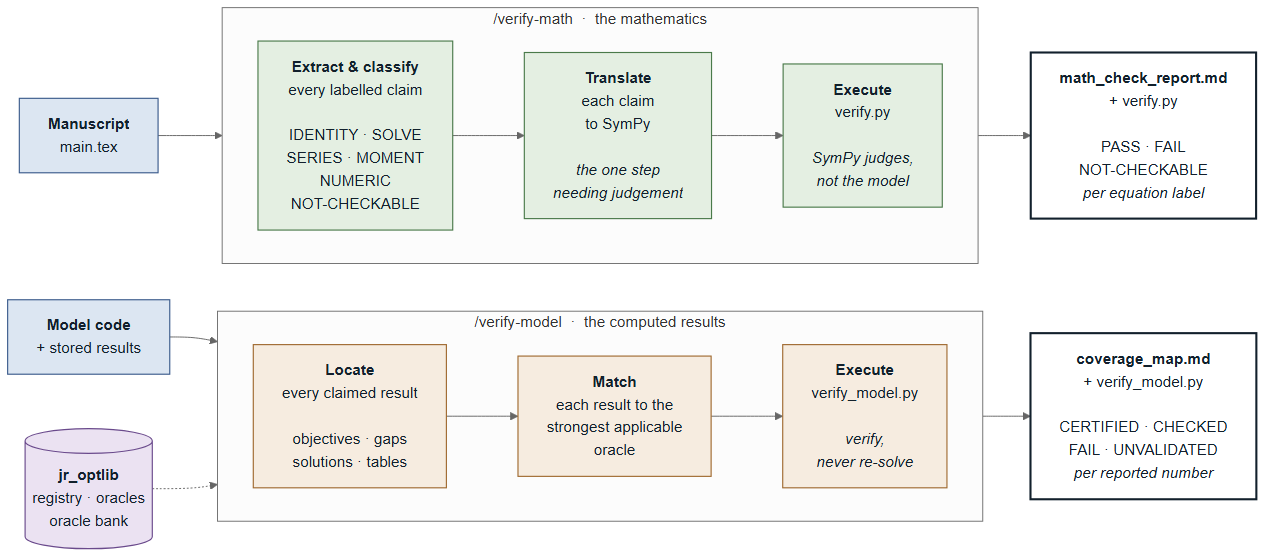
\includegraphics[width=0.86\textwidth]{workflow.png}
  \end{center}
  \vspace{0.5em}
  \begin{columns}[T]
    \begin{column}{0.48\textwidth}
      {\footnotesize Only the \textbf{translation} step needs judgement.
      Everything downstream of it is execution.}
    \end{column}
    \begin{column}{0.48\textwidth}
      {\footnotesize A \FAIL\ sends you back to the manuscript. An \UNV\ sends you to
      \code{jr\_optlib} to add the missing oracle.}
    \end{column}
  \end{columns}
\end{frame}

% =====================================================================
\section{7. Limitations}
\begin{frame}[plain]
  \vfill\centering{\color{dtured}\Large\bfseries 7. Limitations, and why this is the easy version}\vfill
\end{frame}

\begin{frame}{This is not formal verification}
  A proof assistant (Lean, Coq, Isabelle) checks a proof against axioms. Every inference step is
  machine-checked, and the trusted base is a small kernel.
  \vfill
  We do none of that. We check that stated computations are the computations claimed.
  \vfill
  \begin{block}{Three honest limits}
    \begin{enumerate}
      \item \textbf{The translation is trusted.} If the LaTeX is formalised wrongly, the verdict is
            about the wrong claim. Mitigation: the report prints every expression checked.
      \item \textbf{Instantiation is not generality.} Passing at $J \in \{2,3,4\}$ is strong
            evidence, not a proof for all $J$.
      \item \textbf{Reasoning is out of scope.} Limit theorems, existence, uniqueness and
            convergence arguments land in \NC. They always will.
    \end{enumerate}
  \end{block}
\end{frame}

\begin{frame}{Why the easy version is the one worth having}
  \begin{center}
  \begin{tabular}{@{}p{0.24\textwidth}p{0.32\textwidth}p{0.34\textwidth}@{}}
    \toprule
     & \textbf{Proof assistant} & \textbf{What we do} \\
    \midrule
    Guarantee      & the theorem is true & the stated computations are right \\[0.4em]
    Effort         & months per paper, a specialist & minutes per paper, the author \\[0.4em]
    Prerequisite   & the whole theory formalised & a \code{.tex} with labelled equations \\[0.4em]
    Coverage       & total, within what is formalised & partial, and it says which part \\[0.4em]
    Failure mode   & you cannot finish & you get a report with gaps \\[0.4em]
    Adoption       & essentially zero in our field & runs today, on every paper \\
    \bottomrule
  \end{tabular}
  \end{center}
  \vfill
  Full formalisation is stronger and, for applied transport and economics papers, not going to
  happen. A check that runs is worth more than a proof that does not.
\end{frame}

\begin{frame}{Where the errors actually are}
  The errors that reach print in applied work are overwhelmingly \alert{computational, not
  logical}: a dropped term, an inverted formula, a parameter that does not reproduce its table, a
  heuristic reported as an optimum.
  \vfill
  Those are exactly the errors this catches, and exactly the errors a proof assistant would spend
  months getting into position to catch.
  \vfill
  \begin{block}{The trade we are making}
    We give up the guarantee that the theorem is true. We keep the guarantee that the paper says
    what the mathematics says, and we get it cheaply enough to run on everything.
  \end{block}
\end{frame}

% =====================================================================
\section{8. Requirements}
\begin{frame}[plain]
  \vfill\centering{\color{dtured}\Large\bfseries 8. What it takes to install and run}\vfill
\end{frame}

\begin{frame}{What you need}
  \begin{center}
  \begin{tabular}{@{}lp{0.60\textwidth}@{}}
    \toprule
    \textbf{For} & \textbf{You need} \\
    \midrule
    the mathematics & Python with SymPy. That is the whole dependency. \\[0.5em]
    the results     & Python with NumPy and SciPy, plus \code{jr\_optlib}. Solver extras
                      (PuLP, Gurobi, NetworkX, POT, numba) only if your problem uses them. \\[0.5em]
    the automation  & Claude Code, with the two skills in \code{\~{}/.claude/skills/}. \\[0.5em]
    your paper      & a \code{.tex} file with \code{{\textbackslash}label\{\}} on the equations.
                      The labels are what the report keys to. \\
    \bottomrule
  \end{tabular}
  \end{center}
  \vfill
  No LaTeX toolchain is required for the check itself. No proof assistant. No new file format.
  \vfill
  {\color{slate} A paper with unlabelled equations still works; the report anchors to a short quote
  instead. Labelling them is a five-minute investment that makes the report readable.}
\end{frame}

\begin{frame}{Install and run}
  \begin{block}{Once, per machine}
  {\ttfamily\small
  python -m pip install sympy numpy scipy pyyaml\\[0.3em]
  git clone https://github.com/jepperich69/jr\_optlib\\[0.3em]
  cd jr\_optlib \&\& pip install -e .[test]\\[0.3em]
  pytest\hfill{\color{slate}\# 143 oracle-backed tests}}
  \end{block}
  \begin{block}{Per paper}
  {\ttfamily\small
  /verify-math \ --project Pub\_MyPaper\\[0.3em]
  /verify-model --project Pub\_MyPaper}
  \end{block}
  \vfill
  Both run as background agents and open the report when done. Add \code{-{}-inline} for a small
  file you want checked immediately.
  \vfill
  {\color{slate} Output lands in \code{Pub\_MyPaper{\textbackslash}\_math\_checks{\textbackslash}<timestamp>{\textbackslash}}
  next to the manuscript, not in a temporary directory.}
\end{frame}

\begin{frame}{What to write in the paper}
  The wording matters, because the temptation to overclaim is real.
  \vfill
  \begin{block}{Say this}
    ``Checked against independent oracles: feasibility and objective recomputation, duality
    certificates, differential tests against exact solvers, and metamorphic invariants
    (\code{jr\_optlib@<commit>}).''\\[0.5em]
    For a specific number: ``the reported optimum was certified by a zero duality gap.''
  \end{block}
  \begin{block}{Never say this}
    ``Formally verified.'' ``Proven correct.'' ``Machine-checked proof.''
  \end{block}
  \vfill
  Pin the library commit at submission and freeze it. A shared library that keeps improving and a
  paper that must stay reproducible coexist only if the paper names a SHA.
\end{frame}

% =====================================================================
\section{9. Conclusion}
\begin{frame}[plain]
  \vfill\centering{\color{dtured}\Large\bfseries 9. Conclusion}\vfill
\end{frame}

\begin{frame}{Conclusion}
  \begin{enumerate}\itemsep0.7em
    \item \textbf{Checking is cheaper than deriving.} That asymmetry is what makes routine
          verification affordable, and it is the only reason this works.
    \item \textbf{The model translates; the machine judges.} No verdict is ever an opinion.
    \item \textbf{Coverage is part of the output.} \NC\ and \UNV\ are first-class verdicts. A
          report that hides its own boundary is worth less than none.
    \item \textbf{It finds real things.} Three inconsistent calibrations in our own manuscript.
          One unstated side condition in Kahneman and Tversky.
    \item \textbf{It is not formal verification, and does not need to be.} It catches the errors
          that actually reach print, at a cost low enough to run on every paper.
  \end{enumerate}
\end{frame}

\begin{frame}{Where to start}
  \begin{itemize}\itemsep0.8em
    \item Pick the paper you are least sure about. Run \code{/verify-math --project <name>}.
    \item Read the \NC\ list first. It tells you what you are still carrying alone.
    \item If a result has no applicable oracle, that is a gap in \code{jr\_optlib}, not a dead end.
          Adding the oracle once serves every later paper.
    \item Ship \code{verify.py} with the submission. A referee who can run your check is a referee
          you have already answered.
  \end{itemize}
  \vfill
  \begin{center}
  {\color{slate}Reports, scripts and raw output for everything shown:\\
  \code{AI\_auto{\textbackslash}literature{\textbackslash}verification\_demo{\textbackslash}KT1979{\textbackslash}}\\
  \code{Publikationer{\textbackslash}<project>{\textbackslash}\_math\_checks{\textbackslash}}\ \ and\ \ \code{\_model\_checks{\textbackslash}}}
  \end{center}
\end{frame}

\end{document}
